\chapter{A rational choice theory}
While having been criticized for being unsuited to model economic choices made by human beings, a neoclassical economic model of utility maximization can be well-suited to analyze a system such as the one we are interested in. Namely, in practice the making of these choices will be automated and executed by a program well able to quantify utility. Moreover, notice that the model developed below assumes only agents' ability to order different utilities rather than calculate their magnitudes.

\section{Notation}
We will start developing our model by considering a market $M := \{ A | A \ \text{is an agent} \}$ where a unitary good $v$, which has value and can be created by doing one unit of work $w$, is traded. Denote by $V_A$ the set of all $v$ owned or consumed by $A$ and by $W_A$ all units of work $A$ has performed. All agents are able to transact in an atomic, costless manner. Transactions are ordered in time and record a single $v$ being sold by agent $B$ to agent $A$ as transaction $T = (A, p(v), B)$ where $p(v) \in \mathds{R}_{>0}$ denotes the price of $v$. All past transactions are recorded in a history $H$, of which we will for now assume that it is complete and available to all agents in $M$. When a transaction $T$ is appended to history $H$, we denote this by $H + T$. The total number of transactions in $H$ is denoted by $|H|$.

All agents $A \in M$ have a reputation function $r_A: (M \times \mathcal{H}) \to \mathcal{R} = (B, H) \mapsto r_A(B | H)$ where $\mathcal{R}$ denotes the set of possible reputations and $\mathcal{H}$ denotes the set of possible histories $H$. We now define $r_M: (M \times \mathcal{H}) \to \mathcal{R}$ as
\[(A, H) \mapsto \max_{B \in M \setminus \{ A \}} r_B(A | H),\]
the highest reputation assigned by any market member.

We denote by $u^R_A: \mathcal{R} \to \mathcal{U}$ the utility $A$ derives from reputation $r \in \mathcal{R}$, and by $u^V_A: V \to \mathcal{U}$ the utility $A$ derives from valueable $v$. We assume that a unit of work performed by $A$ costs utility $u^W_A$, while a $v$ received lets $A$ enjoy a positive $u^V_A$. The total utility of agent $A$ is now denoted by $u^T_A: \mathcal{H} \to \mathcal{U} = u^R_A + \sum_{v \in V_A} u^V_A(v) + \sum_{w \in W_A} u^W_A(w)$. $\mathcal{R}$ and $\mathcal{U}$ are totally ordered, while for $u^R_A$ we have $x > y \in \mathcal{R} \Rightarrow u^R_A(x) > u^R_A(y)$. Naturally, we suppose that agents in $M$ attempt to maximize their $u^T$ by taking part in the right transactions.

\section{Interpretation}
In such a market $M$, an agent $A$'s reputation depends on the entire history $H$. We can view $A$'s reputation $r_M(A|H)$ as a measure of $A$'s future ability to do create transactions in the network. The price $p(v)$ that two agents might agree upon will depend on the the utility they derive from the valueable $v$ transfered and the change in assigned reputation by the market after this transaction. The reputation of $A$ will influence its ability to participate in $M$ in the future. In this way, the utility derived from $v$ and utility derived from $A$'s reputation represent $A$'s short- and long-term interests respectively.

As is common in micro-economics, we can visualize an agent's trade-off between these short- and long-term interests. On the horizontal axis we measure $|V|$, while on the vertical axis we measure $A$'s reputation. In the case where $u_A^R$ and $u_A^V$ are continuous, we can draw utility level-curves such as in Figure \ref{fig:utility_curves}.

\begin{figure}
	\centering
	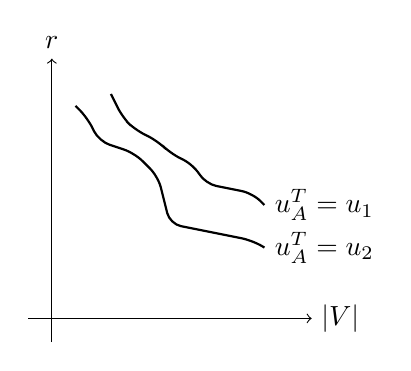
\begin{tikzpicture}[scale=3]
		\draw[->] (-0.1, 0) -- (1.1, 0) node[right] {$|V|$};
		\draw[->] (0, -0.1) -- (0, 1.1) node[above] {$r$};
		
		\draw[thick, rounded corners] (0.1, 0.9) -- (0.15, 0.85) -- (0.2, 0.75) -- (0.35, 0.7) -- (0.45, 0.6) -- (0.5, 0.4) -- (0.6, 0.38) -- (0.65, 0.37) -- (0.75, 0.35) -- (0.85, 0.33) -- (0.9, 0.3) node[right] {$u_A^T = u_2$};
		\draw[thick, rounded corners] (0.25, 0.95) -- (0.3, 0.85) -- (0.35, 0.8) -- (0.45, 0.75) -- (0.5, 0.7) -- (0.6, 0.65) -- (0.65, 0.57) -- (0.75, 0.55) -- (0.85, 0.53) -- (0.9, 0.48) node[right] {$u_A^T = u_1$};
	\end{tikzpicture}
	\caption{Utility curves for agents in $M$. We have $u_1 > u_2$.} \label{fig:utility_curves}
\end{figure}

\subsection{Transaction condition}
We are now ready to formulate a simple transaction condition for agent $A$. Its utility will increase by doing a transaction $T = (A, p(v), B)$ if $u^T_A(H + T) > u^T_A(H)$, or
\[u^R_A(r_M(A|H + T)) + u_A(v) > u^R_A(r_M(A|H)).\]
Note that this condition isn't dependent on $r_A$. This implies that in deciding which trades to perform, an agent's own measure of reputation is irrelevant: it only matters how an agent thinks the rest of the market perceives its actions. In this way, taking the $u_A$'s as given, $A$'s behavior is governed completely the $r$ used by the $B \in M \setminus \{ A \}$. Once a certain reputation function is used by a large fraction of participants, all are incentivized to use it; reestablishing the status quo. For this reason, we'll from now on assume that all agents use the same reputation function $r$ to calculate reputations from $H$.

\section{Conditions for a system of trust}
A question of great importance is which function $r$ to use. Before we dive deeper into this question, we must ask ourselves what behaviors it should generate from agents. An entire chapter is dedicated to this problem (Chapter \ref{chapter:reputation}). For now, we'll only state a requirement that the system as a whole should, at least, achieve.

\subsection{Total contribution and "leakage"}
We first define for agents $A \in M$ the function $\sigma_A: \mathcal{H} \to \mathds{Z} = |W_A| - |V_A|$, the net amount of work performed by $A$. Clearly we would like many agents to have $\sigma \geq 0$, but we will not pursue individual behavior further in this section. Instead, we will consider the summed net contribution of all active agents $A$:
\[L_M(H) := \sum_{A \in M} \sigma_A(H).\]
We call $L_M$ the "leakage" occurring in $M$. It represents the work performed by active agents which is lost to agents that have become inactive. For $M$ to function properly, don't want $L_M$ to become too large. As such, a desirable property of this system is that $\lim_{|H| \to \infty} L_M(H) < \infty$, implying that the amount of lost resources rapidly decreases towards zero over time.

In section \ref{section:requirements_reputation} we will consider several ways in which agents can manipulate the system. We will find that some intuitive functions $r$ don't satisfy the finite leakage property in those cases.

\section{Comparison to a classical market}
It is worth noting a fundamental difference with neoclassical micro-economic analysis of choice theory. In a typical micro-economical market, all buyers and sellers are anonymous. When a product is traded at equilibrium price, participants could first buy the product, and sell it after (or vice-versa) with no change to their money, products or utility. In contrast, consider the decision faced by an agent $A$ in our market $M$. This agent doesn't pay with money, but with its reputation. As soon as $A$ buys the product, $A$'s reputation changes which influences its ability to sell the product after. The same applies for the reverse order of actions: as soon as $A$ sells the product, its reputation changes influencing $A$'s ability to buy it back later.
